% !TEX root = ../thesis-example.tex
%
\chapter{Hypothesis and objectives}
\label{sec:problematic}

\cleanchapterquote{Le fait de rêver est sans doute une des données, plus nombreuses qu'on ne le pense, qui, mieux encore que le soleil ou la pluie, placent les hommes de tout climat, de toute époque et de toute condition devant des problèmes identiques.}{Roger Caillois}{L'incertitude qui vient du rêve, 1956}

\section{The role of arousals on DRF variability}
\label{sec:problematic:arousals}

\section{Influence of sleep inertia on DRF}
\label{sec:problematic:inertia}

\section{Sleep and dream habits in French students}
\label{sec:problematic:survey}

Epidemiological investigations in healthy subjects combining questions on both sleep and dreaming are relatively rare. Such measures are yet necessary to establish and keep up to date sleep and dream norms in the general population. Of particular interest is the college population, which is more at risk of suffering from sleep difficulties than the general population \citep{buboltz_sleep_2001, curcio_sleep_2006, forquer_sleep_2008, lund_sleep_2010}.

In order to recruit participants for our fMRI sleep study (section \ref{sec:problematic:inertia}), we have sent an announcement to several mailing lists of students from Lyon University. The announcement comprised a link to an online questionnaire about sleep and dream habits that participants had to fill out. The analysis of the responses provided up-to-date data on sleep and dream habits of a large sample of French college students, pertaining to different academic fields (i.e. humanities, science, medicine). Because our survey included relatively rare questions (e.g. frequency of recurrent and lucid dreams, sleepwalking, sleep-talking, sleep agitation), and thanks to a large sample of students including much more males than in previous studies (i.e. more than one third), we believe that this study will make a significant contribution to the limited number of previous epidemiological studies on sleep and dream habits of students.

\section{Contribution of day-residues and mundane waking-life events to dream content}
\label{sec:problematic:wle}

\section{An open-source software for sleep scoring and analysis}
\label{sec:problematic:software}

\subsection{Genesis and purpose}
\label{sec:problematic:software:genesis}

During my PhD thesis, I have been working extensively on polysomnographic sleep recordings, notably to score sleep microstructural events (e.g. arousals, rapid eye movements; see section \ref{sec:problematic:arousals}) and sleep stages (see section \ref{sec:problematic:inertia}). Traditionally, the scoring of sleep micro- and macro-structure is done visually and requires therefore a considerable investment of time and effort, in addition with being subject to both inter and intra-rater variability. Sleep scoring can also be done using automatic methods which have the advantage of being fast, reproducible and with generally good agreement with visual scoring \citep{berthomier_automatic_2007, lajnef_learning_2015}. Yet automatic scoring is far from being widespread and most sleep laboratories still rely on visual scoring, using either commercial softwares or in-house packages. In many cases, these softwares come with their own data and hypnogram file formats, and this heterogeneity can represent a substantial obstacle for sharing of algorithms and sleep data across laboratories or clinics. Some of the very few existing and up-to-date open sources alternatives allowing reading and scoring of sleep data are \fnurl{Phypno}{https://pypi.python.org/pypi/phypno} and \fnurl{SpiSOP}{http://www.spisop.org/}, yet they do not include graphical integration of automatic detection and are largely based on command-line options, which are hardly accessible for users with little or no programming knowledge.

It appears that there are currently no free, open-source and easy-to-use software capable of reading several file formats (both for data and hypnogram), and integrating automatic detection of sleep features within the graphical interface. Therefore, I developed during my PhD thesis an open-source software capable of filling this gap. At first intended for my personal use, it soon extended into a fully developed and comprehensive software, partly thanks to the help of my fellow PhD student \fnurl{Etienne Combrisson}{https://etiennecmb.github.io/}. This software was integrated into a broader neuroscientific suite named \fnurl{Visbrain}{http://visbrain.org/}, and the specific sleep module was named \textit{SLEEP}.

The primary aim of \textit{SLEEP} is to provide a fast and intuitive graphical user interface (GUI) to visualize and score polysomnographic sleep recordings. In order to be widely disseminated, the software must support a large range of data file formats, both proprietary (e.g. BrainVision) and public (e.g. European Data Format). It should also be able to handle the great heterogeneity in hypnogram formats (e.g. sampling frequency of the hypnogram, values assigned to each sleep stage). Finally, to provide a significant scoring aid, the software should include several automatic detection algorithms (e.g. spindles, K-complexes, slow-waves) and several signal processing tools (e.g. filtering, referencing). If these conditions are respected, we believe that this software could represent a major methodological development in the field of sleep research.

\section{Summary}
\label{sec:problematic:summary}

\begin{figure}[htb]
	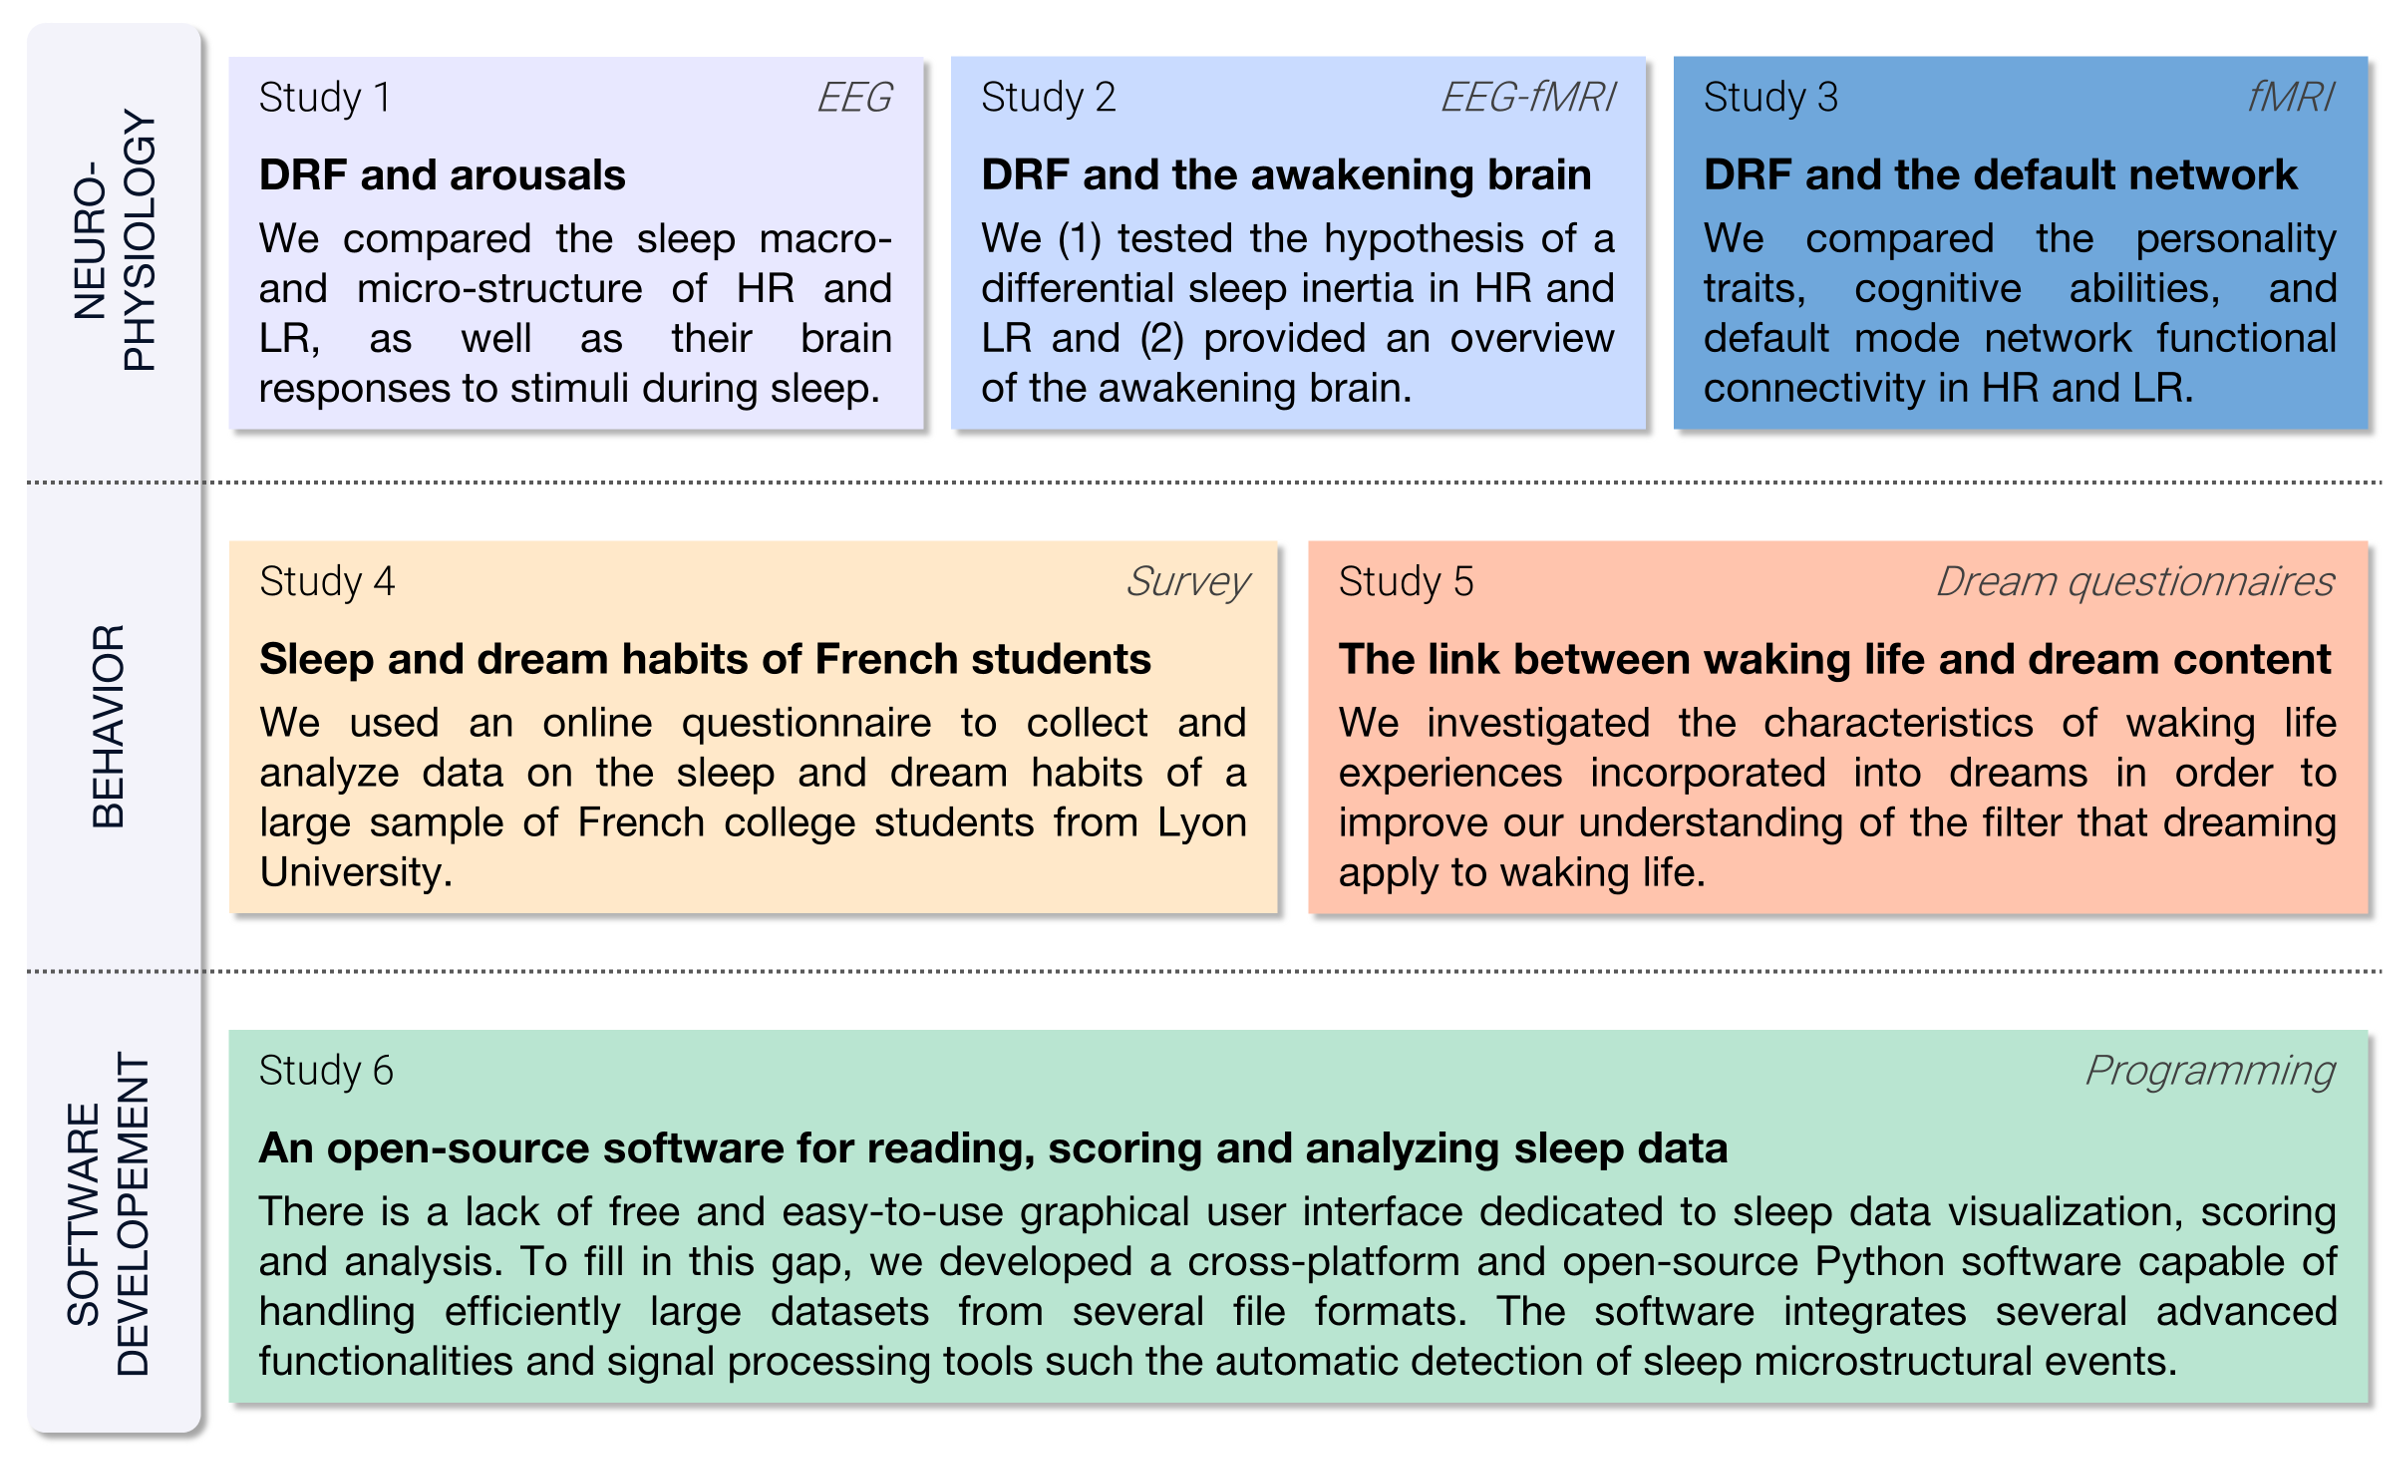
\includegraphics[width=\textwidth]{Fig/Intro/Intro_Problematics/Intro_Problematics.png}
	\caption[Summary of the studies conducted in this thesis]{Summary of the studies conducted in this thesis. In the first two studies, we investigated the neurophysiological correlates of dream recall frequency (DRF) with regards to nocturnal arousals and sleep inertia respectively. Studies 3 is an epidemiological survey of the sleep and dream habits in French college students from Lyon University. In study 4, we conducted a close analysis of the links between waking-life and dream content, with a special emphasis on the incorporation of remote and / or mundane memories. Finally, study 5 relates to the ongoing development of an open-source software to visualize, score and analyze polysomnographic sleep recordings.}
	\label{fig:intro:problematics-summary}
\end{figure}
